\documentclass[ncrna,article,submit,moreauthors,pdftex,10pt,a4paper]{mdpi}

\usepackage{color}
\usepackage[utf8]{inputenc}

\Title{Supplementary File 1}
\Author{}
\address{}

\begin{document}
\section{Methods}
\subsection{Gene structure analysis}

Fig. \ref{comparison} shows the distribution of introns per gene between the dataset and GENCODE v19. We compared the number of introns of every gene from the dataset as we calculated with the same genes as found in GENCODE. Although a similarity could be noticed, we computed a number of genes to have higher number of introns than in GENCODE.
%\clearpage
\begin{figure}[H]
 \centering
 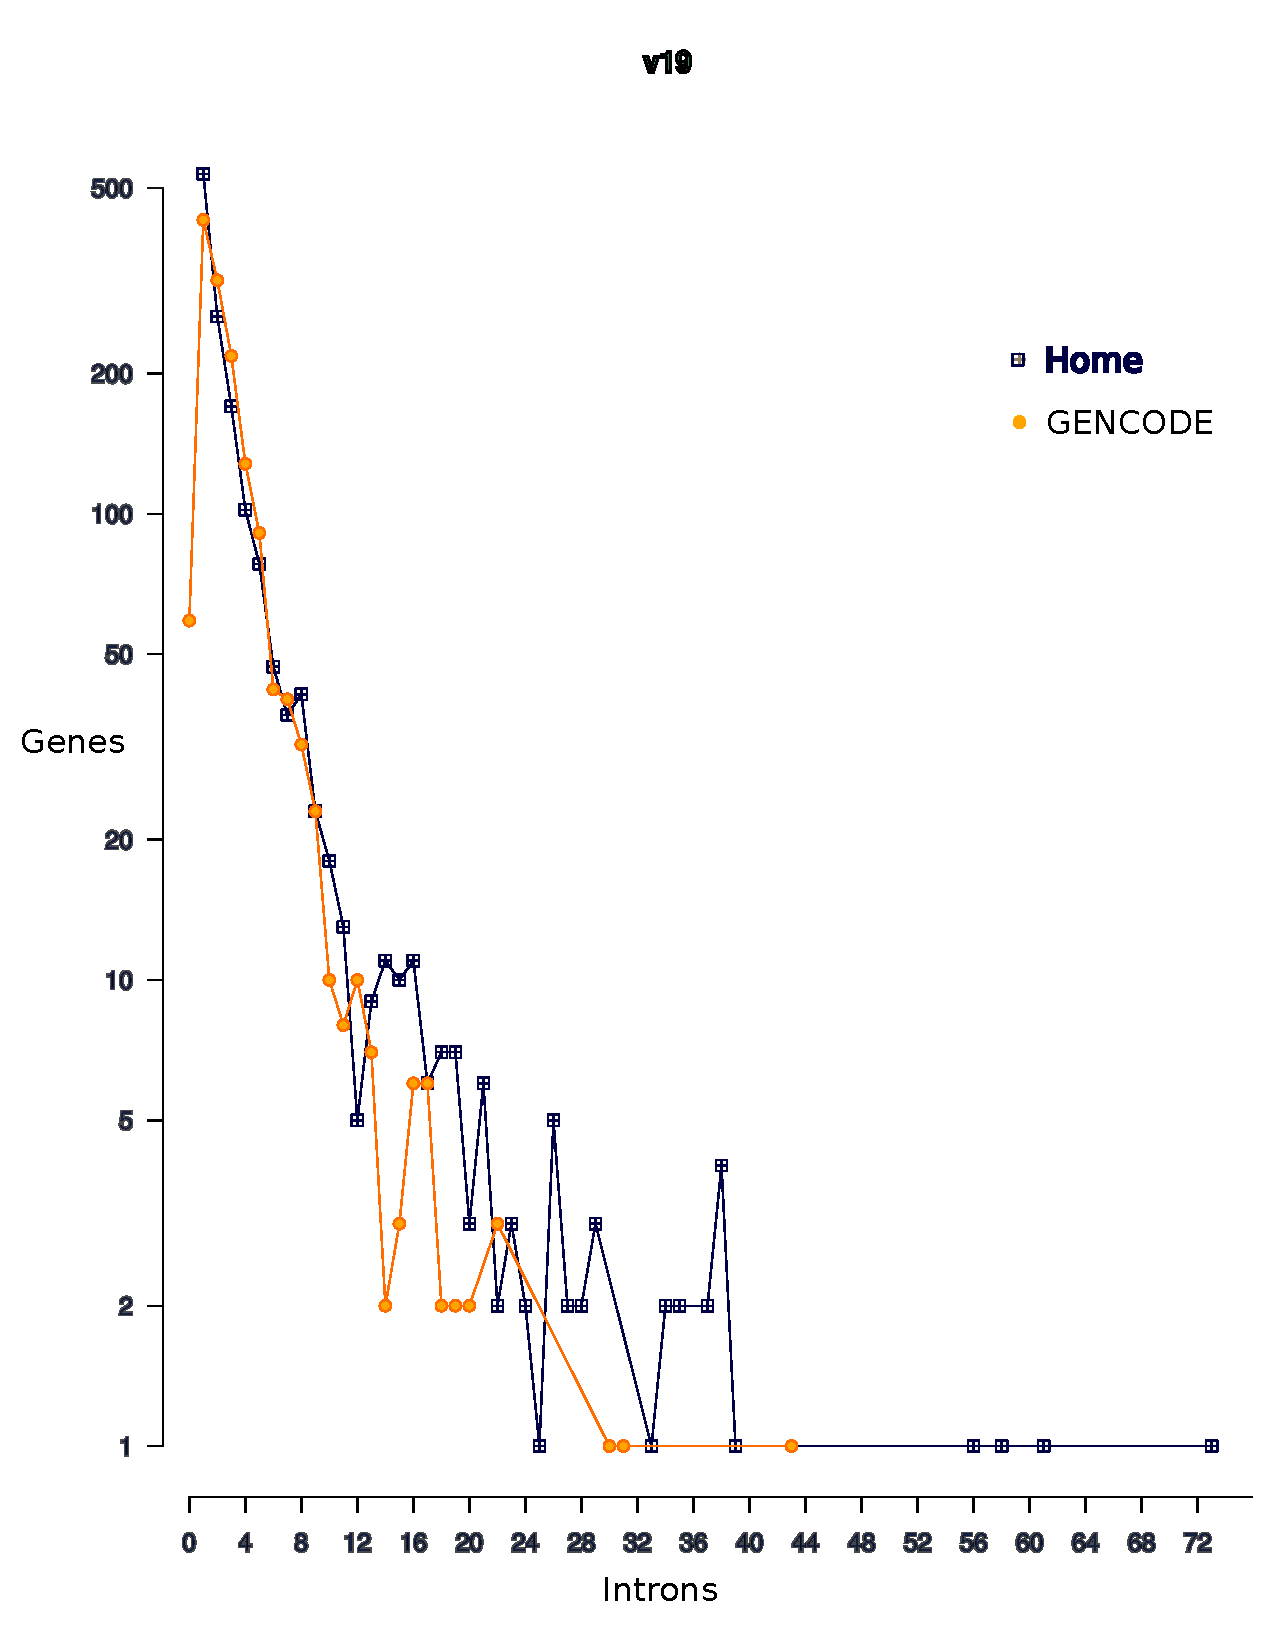
\includegraphics[height = 12 cm, width=14 cm]{comparison_plot_2}
 \caption{The annotations of the lincRNAs from the RNA-Seq data were compared against the annotations of the same lincRNAs found in GENCODE v.19. A considerable number of genes having more introns than reported in GENCODE is shown here.}
 \label{comparison}
\end{figure}

\subsection{Computation of the intersection set}

Our dataset comprises of 5,257 long intergenic noncoding RNA (lincRNA) genes. We compared this set of the genes to the annotation in GENCODE v.7\cite{harrow2012}, v.19 and v.24. We calculated 9,580 genes in GENCODE v.7 (although the authors reported 9,640 lncRNA genes).  This version of GENCODE reports 5,058 lincRNA genes with 8,154 transcripts. The intersection locus had 3,926 genes and 4,563 transcripts annotated in GENCODE v.7. We have also found that mean of exons is 2 according to the annotation in v.7 for the subset of lincRNAs that we have used.

GENCODE v24 reports 15,941 lncRNA genes, among them 7,674 are lincRNAs having 12,656 transcripts. We calculated 4,961 genes from our dataset that are annotated in GENCODE v24. This subset of genes contains 7,487 transcripts. The mean of exons is slightly above 2.

\bibliographystyle{mdpi}
\bibliography{references}

\end{document}
